\documentclass{article}
\usepackage{amsmath}
\usepackage{tikz}

\begin{document}

\begin{figure}[h]
    \centering
    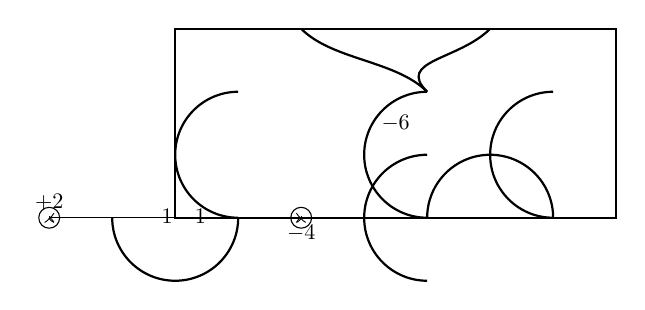
\begin{tikzpicture}[scale=0.8, every node/.style={transform shape}]
        % Draw the 3-line graph
        \node[draw,circle] at (-2,0) (A) {};
        \node[draw,circle] at (2,0) (B) {};
        
        % Draw the edges with labels
        \draw[->] (A) -- node[above] {$+2$} (A |- B);
        \draw[->] (B) -- node[below] {$-4$} (B |- A);
        \draw[->] (A) -- node[left] {$-1$} (B |- A);
        \draw[->] (B) -- node[right] {$-1$} (A |- B);
        
        % Draw the 3-sphere graph (right side)
        \draw[thick] (0,0) rectangle (7,3);
        \draw[thick] (0,3) -- (7,3);
        \draw[thick] (0,0) -- (1,0);
        \draw[thick] (1,3) -- (7,3);
        \draw[thick] (1,0) arc (0:-180:1);
        \draw[thick] (6,0) arc (0:180:1);
        \draw[thick] (4,1) arc (90:270:1);
        \draw[thick] (6,2) arc (90:270:1);
        \draw[thick] (4,2) arc (90:270:1);
        \draw[thick] (1,2) arc (90:270:1);
        \draw[thick] (1,3) -- (2,3);
        \draw[thick] (6,3) -- (5,3);
        \draw[thick] (2,3) .. controls (2.5,2.5) and (3.5,2.5) .. (4,2);
        \draw[thick] (5,3) .. controls (4.5,2.5) and (3.5,2.5) .. (4,2);

        % Add labels for the twist
        \node at (3.5,1.5) {$-6$};
    \end{tikzpicture}
    \caption{Graph diagram for the sequence \(3^\ell 5^\ell 1^+\), and its corresponding 3-line graph, where the twist of the middle edge has been changed by \(-6\) from the case shown in Figure \ref{3-sph-graphs}.}
    \label{fig:3line_graph_with_twist}
\end{figure}

\end{document}